\documentclass{beamer}

\usetheme{Singapore}
\setbeamertemplate{frametitle}[default][left]
\usepackage[utf8]{inputenc}
\usepackage{default}


\newtheorem{df}{Definition}
\newtheorem{thr}{Theorem} %[section]
\newtheorem{pp}{Proposition}

\newtheorem{lm}{Lemma}[thr]


\newcommand{\insertfigure}[3] {

\begin{minipage}[b]{#2\linewidth}
    \includegraphics[width=#2\linewidth]{#1} 
    \caption{#3} 
\end{minipage} }

\newcommand{\insertf}[2]{\insertfigure{#1}{0.9}{#2}}


%insertpicture in beamer
\newcommand{\insertpicture}[2]{
\begin{center}
  \begin{figure}
    \insertf{#1}{#2}
 \end{figure}
\end{center}
}


%tikz
\usepackage{tikz}
\usetikzlibrary{arrows,backgrounds,calc,trees,shapes,snakes,automata,backgrounds,petri,matrix}


\newcommand{\cmdtikz}
{
\tikzstyle{transition}=[circle,draw=black!75,minimum size=1cm]
  \tikzstyle{etou}=[transition,circle,fill=blue!75]
  \tikzstyle{check}= [transition,regular polygon,regular polygon sides=6,fill=red!75]
  \tikzstyle{store}= [transition,diamond,fill=green!75]
  \tikzstyle{move}= [transition,rectangle,fill=yellow!75]
  \tikzstyle{expl}= [transition,rectangle]
 }
\newcommand{\st}[2]{\node [store] (#1) [#2]{$Store$}}
\newcommand{\mv}[2]{\node [move] (#1) [#2]{$Move$}}
\newcommand{\expl}[3]{\node [expl] (#1) [#2]{#3}}

\newcommand{\et}[3]{\node [etou] (#1) [#2]{#3 $\wedge$}}
\newcommand{\ou}[3]{ \node [etou] (#1)  [#2] {#3 $\vee$}}

\newcommand{\eq}[3]{\node [check] (#1) [#2]{$eq_{#3}$}}
\newcommand{\peq}[3]{\node [check] (#1) [#2]{ $\overline{eq_{#3}}$}}
\newcommand{\tl}[3]{\node [check] (#1) [#2]{ $#3$}}
\newcommand{\ntl}[3]{\node [check] (#1) [#2]{ $\overline{#3}$}}
\newcommand{\rt}[1]{edge [pre] (#1)}
\newcommand{\etat}[2]{\node [transition,regular polygon,regular polygon sides=4] (q#1) [#2]  {$q_{#1}$}}

%insert tikz in beamer
\newcommand{\inserttikz}[2]{
\begin{center}
  \begin{figure}
    \scalebox{0.6}{
    \begin{tikzpicture}[node distance=2cm,>=stealth',bend angle=45,auto]
    \cmdtikz
    #1
\end{tikzpicture}

}

\caption{#2}
\end{figure}
\end{center}
}



% highlight edge :

\newcommand{\highe}[4]{\only<{#1}> {\draw[ultra thick,->, %Regular stuff
preaction={%But before that
draw,#2,-,% Draw yellow without any arrow head
double=#2,
double distance=1\pgflinewidth,
}] (#3) to (#4);
}
}

\newcommand{\hye}[3]{\highe{#1}{yellow}{#2}{#3}}

%highlight thread
\newcommand{\hyt}[2]{
\only<#1> {
\fill[yellow,opacity=0.5] \convexpath{#2.west, #2.east}{15pt};

}
}

%conex hull
\pgfdeclarelayer{background}
\pgfsetlayers{background,main}


\newcommand{\convexpath}[2]{
[   
    create hullnodes/.code={
        \global\edef\namelist{#1}
        \foreach [count=\counter] \nodename in \namelist {
            \global\edef\numberofnodes{\counter}
            \node at (\nodename) [draw=none,name=hullnode\counter] {};
        }
        \node at (hullnode\numberofnodes) [name=hullnode0,draw=none] {};
        \pgfmathtruncatemacro\lastnumber{\numberofnodes+1}
        \node at (hullnode1) [name=hullnode\lastnumber,draw=none] {};
    },
    create hullnodes
]
($(hullnode1)!#2!-90:(hullnode0)$)
\foreach [
    evaluate=\currentnode as \previousnode using \currentnode-1,
    evaluate=\currentnode as \nextnode using \currentnode+1
    ] \currentnode in {1,...,\numberofnodes} {
-- ($(hullnode\currentnode)!#2!-90:(hullnode\previousnode)$)
  let \p1 = ($(hullnode\currentnode)!#2!-90:(hullnode\previousnode) - (hullnode\currentnode)$),
    \n1 = {atan2(\x1,\y1)},
    \p2 = ($(hullnode\currentnode)!#2!90:(hullnode\nextnode) - (hullnode\currentnode)$),
    \n2 = {atan2(\x2,\y2)},
    \n{delta} = {-Mod(\n1-\n2,360)}
  in 
    {arc [start angle=\n1, delta angle=\n{delta}, radius=#2]}
}
-- cycle
}



\begin{document}

\section{Introduction.}

\begin{frame}{Coventry}
  \insertpicture{pictures/coventry.jpg}{Coventry}
\end{frame}
\begin{frame}{History.}
\begin{columns}[T] % align columns
\begin{column}{.48\textwidth}
\begin{figure}
  
  \insertf{coventryb.jpg}{Coventry bombed.}
  \pause
  \insertf{pictures/crypto.jpg}{Crypto.}
  \pause

 
\end{figure}
\end{column}%
\begin{column}{.40\textwidth}

\begin{figure}
  
  \insertf{pictures/Sherlock.jpg}{Sherlock.}
  \pause
  \insertf{pictures/consp.jpg}{Conspiracy.}
  
 
\end{figure}

  \end{column}%
\end{columns}

\end{frame}

\begin{frame}{Emptyness decidability on Alternative Register Automata.}
\begin{columns}[T] % align columns
\begin{column}{.48\textwidth}
\begin{figure}
  
  \insertf{coventryb.jpg}{Sylvain.}
  \pause
  \begin{itemize}
   \item Preuve 1 \pause
   \item Preuve 2 \pause
   \item Preuve 3 \pause
  \end{itemize}

 
\end{figure}
\end{column}%
\begin{column}{.40\textwidth}

\begin{figure}
  
  \insertf{pictures/Sherlock.jpg}{Ranko.}
  \pause
  \insertf{pictures/consp.jpg}{Martin.}
  
 
\end{figure}

  \end{column}%
\end{columns}

\end{frame}

\section{Data words and register automata.}
  
\begin{frame}{Data words.}
  TODO
\end{frame}


\begin{frame}{Definition of our automatas, configurations and a runs.}
\inserttikz{

\pause

\node [transition,regular polygon,regular polygon sides=4] (q1)  {$q_1$};
\etat {2} {below of=q1};
\etat {3} {below of=q2};

\node (invi2) [draw= none, left of=q1] {};

\pause
\ou {ou}{right of= q1}{}
\rt {q1};

\pause
\etat{5}{right of= ou}
  \rt {ou};
\etat{4}{above of= q5}
  \rt {ou};
  
\pause
\et {et}{right of= q2}{}
\rt {q2};
\etat{6}{right of= et}
  \rt {et};
\etat{7}{below of= q6}
  \rt {et};
\et {et2}{right of= q6}{}
\rt {q6};
\etat{9}{right of= et2}
  \rt {et2};
\etat{8}{above of= q9}
  \rt {et2};

\pause  
\peq{peq}{right of= q4}{1}
\rt{q4};


\eq{eq}{right of= q5}{2}
\rt{q5};


\tl{ta}{right of= q7}{a}
\rt{q7};

\ntl{tb}{right of= q3}{b}
\rt{q3};




\pause
\st{store}{above of= q8}
  \rt {q8};
\etat{10}{right of= store}
  \rt {store};
  
  
\pause
\mv{move}{right of= q10}
\rt {q10};
\etat{11}{below of= move}
\rt {move};

\mv{move2}{right of= q9}
\rt {q9};
\etat{12}{right of= move2}
\rt {move2};


% explaination
\node (invi) [draw= none, left of=q3] {};

\visible<13-16,25-26>
{\expl{t3}{left of = invi}{
  \only<13-16> {$t_3$}
  \only<25-> {$t_4$}
  \only<14-16> {$=(q_3$}
  \only<25-> {$=(q_7$}
  \only<15-> {$,y)$}
  };
}

 \visible<13->
 {\expl{t2}{above of = t3}{$t_2$
  \only<14-24> {$=(q_2$}
  \only<25-27> {$=(q_6$}
  \only<28-31> {$=(q_9$}
  \only<32> {$=(q_{12}$}
 
  \only<15-> {$,y)$}
  };
 }
 
 \visible<13-22,28->
 {\expl{t1}{above of = t2}{
  \only<13-22> {$t_1$} 
  \only<28-> {$t_5$}
  \only<14-18> {$=(q_1$}
  \only<19-20>{$=(q_4$}
  \only<21-22>{$=(q_5$}
  \only<28-29>{$=(q_8$}
  \only<30-31>{$=(q_{10}$}
  \only<32->{$=(q_{11}$}
  \only<15-27> {$,x)$}
  \only<28-29> {$,y)$}
  \only<30-> {$,x)$}
  
  };
 }
 
 \visible<9-> {\expl{rho}{above of= t1}{
 \only<9-> {$\rho =($} 
  \only<10-31> {$a,$}
  \only<11-31> {$x,$}
  \only<32-> {$b,z,$}
 \only<12-> {$\Delta$}
  \only<13-15> {$=\{t_1;t_2;t_3\})$ }
  \only<16-22> {$=\{t_1;t_2\})$ }
  \only<23-24,26-27> {$=\{t_2\})$ }
  \only<25> {$=\{t_2;t_4\})$ }
  \only<28-> {$=\{t_2;t_5\})$ }

 };
}
 %first check
 \hye{16}{q3}{tb}
 \hyt{16}{t3}
 
 %explain ou
 \hyt{18-22}{t1}
 \hye{18-21}{q1}{ou}
 \hye{18-20}{ou}{q4}
 \highe{20}{red}{q4}{peq}
 \hye{18,21}{ou}{q5}
 
 %kill eq
 
 \hye{22-23}{q5}{eq}
 
 %et 
 \hyt{24-25}{t2}
 \hye{24-25}{q2}{et}
 \hye{25}{et}{q6}
 \hye{25}{et}{q7}
 \hyt{25}{t3}
 
 %eq
 \hyt{26}{t3}
 \hye{26}{q7}{ta}
 
 
 %et2
 \hyt{27-28}{t2}
 \hye{27}{q6}{et2}
 
 \hyt{28-}{t1}
 \hye{28}{et2}{q8}
 \hye{28}{et2}{q9}
 
 %store
 \hye{29-30}{q8}{store}
 \hye{30}{store}{q10}
 
 %move
  \hyt{31-}{t2}
  \hye{31}{q10}{move}
  \hye{31}{q9}{move2}
  \hye{32}{move}{q11}
  \hye{32}{move2}{q12}


}
{Example for the definition.}

\end{frame}



\begin{frame}{Example with n = 1.}
\inserttikz{
\node [transition,rectangle] (q0)  {$q0$};
  \mv {1}{below of= q0} 
    edge [pre] (q0);
  \ou {2}{below of= 1} {$q_{a \vee b}:$ } 
    edge [pre] (1);

    %right%
     
   \et {qb}{right of = 2 } {$q_b$ :}
     \rt  {2};
   \tl{tb}{right of= qb}{b}
     \rt {qb};
   \ou {qki}{below of= qb }{$q_{e}$ :} 
     \rt{qb};
   \eq{eq}{below of= qki}{}
     \rt{qki};
   \mv{move2}{right of= qki}
     \rt{qki}
     edge [post] (qb);
   
   
    %left%
    
   \et {qa}{left of = 2 } {$q_a$:}
      \rt {2};
   \tl{ta}{left of= qa}{a}
     \rt {qa};
   \et{qc}{below of= qa }{$q_{ck}$ :}
     \rt{qa};
   \mv{move}{right of= qc}
     edge [post](2)
     \rt{qc};
     
   \st{store}{below of=qc}
    \rt{qc}
    edge [post] (move);
     \peq{peq}{left of= qc}{}
     \rt{qc};
  
  
 

  \begin{pgfonlayer}{background}
  \pause
  %if
  \expl{ca}{left of= ta}{case a};
  \fill[blue,opacity=0.5] \convexpath{ca,ta,qa,qa.south,qa,2}{23pt};
  \pause
  \expl{cb}{right of= tb}{case b};
  \fill[blue,opacity=0.5] \convexpath{2,qb,qb.south,qb,tb,cb}{23pt};
  
  %create
  \pause
  \expl{cs}{below of= store}{create};
  \fill[green,opacity=0.5] \convexpath{qc,store,qc,cs}{23pt};
  %erase
  \pause
  \expl{ck}{below of= eq}{erase};
  \fill[black,opacity=0.5] \convexpath{qki,eq,ck}{23pt};
   
  %kill
  \pause
  \expl{cc}{left of= peq}{kill};
  \fill[red,opacity=0.5] \convexpath{qc,peq,cc}{23pt};
   
  
  \end{pgfonlayer}
}
{$a^nb^m$ with $n \leq m$.}

\end{frame}
\begin{frame}{Example with n.}
\inserttikz{

\tikzstyle{triangleinvi}= [transition,fill=white, regular polygon,regular polygon sides=6,dashed]
 \node [transition,regular polygon, regular polygon sides = 4] (q0)  {$q0$};
 \mv {move}{right of= q0} 
    edge [pre] (q0);
  \st {store}{right of= move}
    \rt {move};    
 \et {big}{right of= store}{}
    \rt{store}
    edge [post,bend right] (move);
 \ou {ou}{right of= big}{$k$ :}
    \rt{big};
 \node (invi6) [circle,dashed,above of=ou] {}
  edge [dashed,pre] (big);
 \node (invi7) [draw=none,below of=ou] {}
  edge [dashed,pre] (big);
 \ou {ou1}{above of= invi6}{$0$ :}
    \rt{big}
    edge [dashed] (ou);
 \node (invi4) [triangleinvi,below right of=ou1] {}
    edge [pre,dashed] (ou1);
 \node (invi5) [triangleinvi,right of=ou1] {}
  edge [pre,dashed] (ou1);
 \ou {oun}{below of= invi7}{$n-1$ :}
    \rt{big}
    edge [dashed] (ou);
 \node (invi2) [triangleinvi,right of=oun] {}
    edge [pre,dashed] (oun);
 \node (invi3) [triangleinvi,above right of=oun] {}
  edge [pre,dashed] (oun);
 
 \node (invi) [draw=none,right of=ou] {};
 \eq {eq}{above right of=invi}{k}
    \rt{ou};
 \peq {peq}{below right of=invi}{k+1}
    \rt{ou};
 
 
  
  

   \begin{pgfonlayer}{background}
  \pause
 %create
  \expl{cr}{below of=store}{create};
  \fill[green,opacity=0.3] \convexpath{move,store.north,store,cr,store,store.north,big}{23pt};
  
  \pause
  %delete
  \expl{dl1}{right of=eq}{delete};
  \fill[black,opacity=0.3] \convexpath{ou,eq,dl1}{23pt};
  
  \pause
  %delete
  \expl{dl2}{right of=peq}{delete};
  \fill[black,opacity=0.3] \convexpath{ou,peq,dl2,peq}{23pt};
  
  \pause
  %for 
  \node (invi2) [draw=none,left of=ou1] {};
   \expl{for}{left of=invi2} {for $k$ from $0$ to $n-1$};
  \fill[blue,opacity=0.3] \convexpath{for.west,for,ou1,big,ou1,ou,oun,big,ou,ou1}{23pt};
  
  
  \end{pgfonlayer}
 
}
{Progressively finer.}

\end{frame}




\section{The main theorem.}


\begin{frame}{Statement of the main theorem, and proposition used.}
\begin{thr}[Main]
 The emptiness problem on $NARA$ is decidable.
\end{thr}
  \pause
 \begin{pp} 
   If  $\rightarrow$ is a transition system effective rdc with respect of $\preceq$, a wqo decidable, then for any finite set $I$ it's possible to compute a finite set $U$ such that
   $\uparrow_\preceq U=\uparrow_\preceq Succ^*_\rightarrow (I)$.
 \end{pp}
\pause
How to use that propostion?:
\begin{itemize}
\pause
 \item $\exists a \in I$\ and $\exists b \in F$ such that $ a \rightarrow^* b $? \pause
 \item compute $U$. \pause
 \item $U \cap F = \emptyset$. \pause
 \item $F$ downward closed.
\end{itemize}


\end{frame}


\begin{frame}{Division theorem into several lemmas.}
 \begin{itemize}
 \item $\preceq$ is a wqo ,
 	\item $\preceq$ is decidable ,
 	\item $\rightarrow$ is effective ,
	\item $\rightarrow$ is rdc with respect to $\preceq$,
 	\item $F$ is downward closed ,
 	\item $F$ is recursive .
  \end{itemize}
\end{frame}



\begin{frame}{An efficient relation order. }

\begin{columns}[T] % align columns
\begin{column}{.5\textwidth}
\begin{df}[rdc]
reflexive downward compatible 
\only<2> {
\begin{tikzpicture}
  \matrix (m) [matrix of math nodes,row sep=2em,column sep=0.5em,minimum width=2em,ampersand replacement=\&]
  {
     \rho \& \preceq \& \rho_2 \\
     \phantom {test }\& \phantom {\preceq} \& \rho_3 \\};
  \path[-stealth]
    %(m-1-1) edge node [left] {($=$)} (m-2-1)
    (m-1-3) edge node [left] {} (m-2-3);
\end{tikzpicture}

}	
\only<3-> {

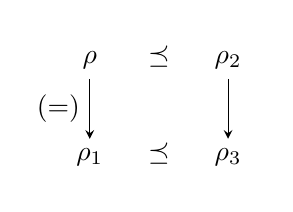
\begin{tikzpicture}
  \matrix (m) [matrix of math nodes,row sep=2em,column sep=0.5em,minimum width=2em,ampersand replacement=\&]
  {
     \rho \& \preceq \& \rho_2 \\
      \rho_1 \& \preceq \& \rho_3 \\};
  \path[-stealth]
    (m-1-1) edge node [left] {($=$)} (m-2-1)
    (m-1-3) edge node [left] {} (m-2-3);
\end{tikzpicture}
}

 
\end{df}


\end{column}%
\begin{column}{.6\textwidth}


\pause
\pause
\begin{df}[$\preceq$] 
  \pause
  \begin{itemize}
    \item [$\equiv$] : $\rho \equiv \rho' \Leftrightarrow \exists f \ f(\rho) = \rho'$. \pause
    \item [$\leq$] : $\rho \leq \rho_2 \Leftrightarrow  \Delta \subseteq \Delta_2 $. \pause
    \item [$\preceq$] $\rho \preceq \rho_2 \Leftrightarrow \exists \rho' \ \rho \equiv \rho' \leq \rho_2$. 
  \end{itemize}
	
\end{df}

  \end{column}%
\end{columns}
\pause
\begin{lm}
  $\rightarrow$ is reflexive downward compatible  with respect of $\preceq$.
\end{lm}
\pause
Explaination : \\\
\only<8>{
\begin{tikzpicture}
  \matrix (m) [matrix of math nodes,row sep=2em,column sep=0.5em,minimum width=2em,ampersand replacement=\&]
   {
     \rho \& \equiv \& \rho' \& \leq \& \rho_2 \\
     \phantom{\exists\rho_1} \&  \phantom{\equiv }\& \phantom{\exists \rho'_1} \&  \phantom{\preceq} \& \rho_3 \\
     };
   \path[-stealth]
%     (m-1-1) edge node [left] {($=$)} (m-2-1)
 %    (m-1-3) edge node [left] {($=$)} (m-2-3)
     (m-1-5) edge node [left] {} (m-2-5);
 \end{tikzpicture}
}

\only<9>{
\begin{tikzpicture}
  \matrix (m) [matrix of math nodes,row sep=2em,column sep=0.5em,minimum width=2em,ampersand replacement=\&]
   {
     \rho \& \equiv \& \rho' \& \leq \& \rho_2 \\
     \phantom{\exists\rho_1} \&  \phantom{\equiv }\& \exists \rho'_1 \&  \leq \& \rho_3 \\
     };
   \path[-stealth]
%     (m-1-1) edge node [left] {($=$)} (m-2-1)
     (m-1-3) edge node [left] {\phantom{($=$)}} (m-2-3)
     (m-1-5) edge node [left] {} (m-2-5);
 \end{tikzpicture}
}

\only<10>{
\begin{tikzpicture}
  \matrix (m) [matrix of math nodes,row sep=2em,column sep=0.5em,minimum width=2em,ampersand replacement=\&]
   {
     \rho \& \equiv \& \rho' \& \leq \& \rho_2 \\
     \phantom{\exists\rho_1} \&  \phantom{\equiv }\& \exists \rho'_1 \&  \leq \& \rho_3 \\
     };
   \path[-stealth]
%     (m-1-1) edge node [left] {($=$)} (m-2-1)
     (m-1-3) edge node [left] {($=$)} (m-2-3)
     (m-1-5) edge node [left] {} (m-2-5);
 \end{tikzpicture}
}

\only<11>{
\begin{tikzpicture}
  \matrix (m) [matrix of math nodes,row sep=2em,column sep=0.5em,minimum width=2em,ampersand replacement=\&]
   {
     \rho \& \equiv \& \rho' \& \leq \& \rho_2 \\
     \phantom{\exists\rho_1} \&  \phantom{\equiv }\& \exists \rho'_1 \&  \preceq \& \rho_3 \\
     };
   \path[-stealth]
%     (m-1-1) edge node [left] {($=$)} (m-2-1)
     (m-1-3) edge node [left] {($=$)} (m-2-3)
     (m-1-5) edge node [left] {} (m-2-5);
 \end{tikzpicture}
}


\only<12>{
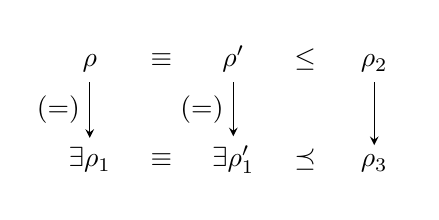
\begin{tikzpicture}
  \matrix (m) [matrix of math nodes,row sep=2em,column sep=0.5em,minimum width=2em,ampersand replacement=\&]
   {
     \rho \& \equiv \& \rho' \& \leq \& \rho_2 \\
     \exists\rho_1 \&  \equiv \& \exists \rho'_1 \&  \preceq \& \rho_3 \\
     };
   \path[-stealth]
     (m-1-1) edge node [left] {($=$)} (m-2-1)
     (m-1-3) edge node [left] {($=$)} (m-2-3)
     (m-1-5) edge node [left] {} (m-2-5);
 \end{tikzpicture}
}
\end{frame}

\begin{frame}{Projections: $\Delta^k(x)$ and $g^k_\Delta(S)$.}
 TODO
\end{frame}
\begin{frame}{$\preceq$ is a well quasi order.}
 \begin{itemize}
  \pause
  \item Reflexive and transitive \pause : take $\rho$ and look for $\rho_i \preceq \rho_j$ \pause
  \item Data $\infty$, Threads $\infty$ \pause : use $g^k_{\Delta}(S)$.  \pause
  \item Still infinite \pause : use cardinals. \pause
  \item $\forall S, \forall k $: use Dickson's lemma. \pause
  \item $\Delta_i$ and $\Delta_j$ \pause $\exists f $ $f(\Delta_i) \subseteq \Delta_j$ \pause
  \item But what about $(a,x)$? \pause : project on $(a,\Delta(x))$. \pause
  \item Found $\rho_i$ and $\rho_j$ \pause $\exists f $ $f(\rho_i) \preceq \rho_j$. \pause 
  \item $\preceq$ is a well quasi order.
 \end{itemize}

\end{frame}

\begin{frame}{Last lemmas.}
\begin{lm} 
  $\preceq$ is decidable.
\end{lm}
\pause
\begin{lm} 
  $\rightarrow$ is effective.
\end{lm}
\pause
\begin{lm} 
  $F$ is downward closed. 
\end{lm}
\pause
\begin{lm} 
  $F$ is reccursive.
\end{lm}

\end{frame}




\section{Conclusion}


\begin{frame}{Other part of the internship.}
 TODO
\end{frame}

\begin{frame} {Conclusion}
  TODO
\end{frame}

%uk seule
\begin{frame}{Geography}
  \begin{figure}
  
     \begin{center}
	 \includegraphics[width=1\linewidth]{pictures/uk.pdf}
	 
  
    \end{center}

    
  \end{figure}

\end{frame}

%coventry

\begin{frame}{Geography}
  \begin{figure}
  
     \begin{center}
	 \includegraphics[width=1\linewidth]{pictures/coventryalone.pdf}
	 
  
    \end{center}

    
  \end{figure}

\end{frame}


%rugby


\begin{frame}{Geography}
  \begin{figure}
  
     \begin{center}
	 \includegraphics[width=1\linewidth]{pictures/covr.pdf}
	 
  
    \end{center}

    
  \end{figure}

\end{frame}
\begin{frame}{Geography}
  \begin{figure}
  \begin{minipage}[b]{0.8\linewidth}
     \begin{center}
	 \includegraphics[width=0.8\linewidth]{pictures/covr.pdf}
	 
  
    \end{center}

    
  \end{minipage} 
  \end{figure}
  
  \begin{figure}
  \begin{minipage}[b]{0.5\linewidth}
     \begin{center}
	 \includegraphics[width=0.5\linewidth]{pictures/rugby.pdf}
  
    \end{center}

    
  \end{minipage}
   \end{figure}

  \end{frame}
\begin{frame}{Geography}
  \begin{figure}
  \begin{minipage}[b]{0.8\linewidth}
     \begin{center}
	 \includegraphics[width=0.8\linewidth]{pictures/covrl.pdf}
	 
  
    \end{center}

    
  \end{minipage} 
  \end{figure}
  
  \begin{figure}
  \begin{minipage}[b]{0.5\linewidth}
     \begin{center}
	 \includegraphics[width=0.5\linewidth]{pictures/rugby.pdf}
  
    \end{center}

    
  \end{minipage}
   \end{figure}

  \end{frame}
 

\begin{frame}{Geography}
  \begin{figure}
  
  \begin{minipage}[b]{0.7\linewidth}
     \begin{center}
	 \includegraphics[width=0.7\linewidth]{pictures/covrl.pdf}
	 
  
    \end{center}

    
  \end{minipage} 
  \end{figure}
  \begin{minipage}{0.6\linewidth}
  
  \begin{columns}[c] % align columns
\begin{column}{.6\textwidth}
\begin{figure}
  
 \insertf{pictures/rugby.pdf}{Rugby}
  

 
\end{figure}
\end{column}%
\begin{column}{.7\textwidth}

\begin{figure}
  
  \insertf{pictures/saracens.pdf}{Saracens.}
  \pause
 
\end{figure}

  \end{column}%
\begin{column}{.3\textwidth}

\begin{figure}
  Parce que Toulon!!! 
  \insertf{pictures/rct.pdf}
  
 
\end{figure}

  \end{column}%

  \end{columns}

\end{minipage}

\end{frame} 

\begin{frame}{Merci.}
 
\end{frame}



\end{document}
